\section{Detailed Implementation}\label{section:implementation}


\subsection{Simple MDP}

\subsubsection{Simple MDP\ -\ SARSA}

The pseudocode shows how we run SARSA in the simple MDP environtment.
The introduction of simple MDP can be found here (figure\ \ref{fig:simple_mdp}).

\begin{algorithm}
    \caption{Simple MDP\ -\ SARSA}\label{alg:SimpleMDP-SARSA}
    If using Mellowmax, replace `Boltzmann' with `mm' and relpace $\beta$ with $\omega$.\\
    \textbf{Input:} init $Q(s,a) \forall s\in \mathcal{S} \forall a\in \mathcal{A}$, $\alpha$ and $\beta$
    \begin{algorithmic}[1]
        \For{each episode}
            \State{Init $s$}
            \State{$a\sim $ Boltzmann with $\beta$}
            \Repeat{}
                \State{Take action $a$, observe $r,s'$}
                \State{$a'\sim$ Boltzmann with $\beta$}
                \State{$Q(s,a)\leftarrow Q(s,a)+\alpha[r+\gamma Q(s',a')-Q(s,a)]$}
                \State{$s\leftarrow s'$,$a\leftarrow a'$}
            \Until{$s$ is terminal}
        \EndFor{}
    \end{algorithmic}
\end{algorithm}

\subsubsection{Simple MDP\ -\ GVI}\label{sec:simpleMDP_GVI}

The pseudocode below shows how we run generalized value iteration (GVI) in the simple MDP environtment to find the number of fixed points.
We don't know how the paper's authors determine whether > 1 fixed points.
The way we adopt to decide if > 1 fixed points is to try different initial Q values.
If some initial Q values lead to different fixed points, it means > 1 fixed points.
Hence, it's more accurate if more various Q initial values are tried.

\begin{algorithm}
    \caption{Simple MDP\ -\ GVI}\label{alg:SimpleMDP-GVI}
    Consider $s_1$'s two actions' Q values: $Q(s_1,\text{a})$ and $Q(s_1,\text{b})$\\
    Note that $\text{a}$ means action a of $s_1$; $a$ indicates `action`.\\
    \textbf{Input:} softmax operator $\otimes$ (bolz or mm), all pairs of $Q(s_1,\text{a}),\hat{Q}(s_1,\text{b})$ to run, $\alpha$ and $\beta$ or $\omega$
    \begin{algorithmic}[1]
        \State{$\mathcal{Q}\leftarrow\{\}$}  \Comment{$\mathcal{Q}$ stores each trial's convergence fixed point.}
        \State{$\delta\leftarrow 10^{-14}$}
        \For{each initial value pair $Q(s_1,\text{a}),Q(s_1,\text{b})$}
            \Repeat{}
                \For{$a\in \{\text{a},\text{b}\}$}
                    \State{$Q_\text{copy}\leftarrow Q(s_1,a)$}
                    \State{$Q(s_1,a)\leftarrow R(s,a)+\gamma\sum_{s'\in\{s_1,s_2\}}
                            P(s,a,s') \otimes Q(s',\cdot)$}                    
                    \State{$\text{diff}_{a}\leftarrow\max({\text{diff}_a},|Q_\text{copy}-Q(s_1,a)|)$}
                \EndFor{}
            \Until{$\max(\text{diff}_a) < \delta$}
            \State{Push fixed point $(Q(s_1,\text{a}),Q(s_1,\text{b}))$ into $\mathcal{Q}$}
        \EndFor{}
        \State{$N\leftarrow \text{size}(\text{uniq}(\mathcal{Q}))$}
        \If{$N$>1}
            \State{More than 1 fixed points from given initial Q pairs.}
        \Else{}
            \State{No more than 1 fixed points from given initial Q pairs.}
        \EndIf{}
    \end{algorithmic}
\end{algorithm}


\subsubsection{Ramdom MDP\ -\ GVI}

The following pseudocode shows how we run generalized value iteration (GVI) in the randomly constructed MDP environtment to find the number of fixed points.
Similar to\ \ref{sec:simpleMDP_GVI}, here we decide if > 1 fixed points by sampling initial Q values.
Hence, it's more accurate if more various Q initial values are tried.
(More discussion is here [\ref{randomMDP_finding_fixed_points_issue}].)

\begin{algorithm}
    \caption{Ramdom MDPs\ -\ GVI}\label{alg:RandomMDP-GVI}
    \textbf{Input:} softmax operator $\otimes$ (bolz or mm), $N_\text{MDP}$, $N_\text{trial}$, $\alpha$ and $\beta$ or $\omega$
    \begin{algorithmic}[1]
        \Function{ConstructMDP}{}
            \State{$\mathcal{P}:|\mathcal{S}|\times |\mathcal{A}|\times |\mathcal{S}|;\mathcal{R}:|\mathcal{S}|\times |\mathcal{A}|$}
            \State{$|\mathcal{S}|$ sample from $\{2,3,4,5\}$ uniformly at random.}
            \State{$|\mathcal{A}|$ sample from $\{2,3,4\}$ uniformly at random.}
            \State{$\mathcal{P}\sim U[0,0.01], \mathcal{R}\sim U[0,0.01]$}
            \State{Each entry of $\mathcal{P}$ and $\mathcal{R}$ increase a value $\sim\mathcal{N}(1,\sqrt{0.1})$ with prob. 0.5}.
            \State{Each entry of $\mathcal{P}$ and $\mathcal{R}$ increase a value $\sim\mathcal{N}(100,\sqrt{1})$ with prob. 0.1}.
            \State{Normalize $\mathcal{P}$ to be a transition matrix.}
            \State{For each $s$ of $\mathcal{R}$, divide $\mathcal{R}(s,\cdot)$ by $\max(\mathcal{R}(s,\cdot))$ and $\times 0.5$.}
        \EndFunction{}
        \State{$N_\text{nonSingle}\leftarrow 0$}
        \State{$\delta\leftarrow 10^{-14}$}
        \For{$i\leftarrow$ to $N_\text{MDP}$}
            \State{$\mathcal{Q}\leftarrow\{\}$}  \Comment{$\mathcal{Q}$ stores each trial's convergence fixed point.}
            \For{$j\leftarrow$ to $N_\text{trial}$}    
                \State{All value $Q\sim U[0,30]$ }
                \Repeat{} 
                    \For{$s\in\mathcal{S}$}
                        \For{$a\in\mathcal{A}$}
                            \State{$Q_\text{copy}\leftarrow Q(s,a)$}
                            \State{$Q(s,a)\leftarrow R(s,a)+\gamma\sum_{s'\in\mathcal{S}}
                                    P(s,a,s') \otimes Q(s',\cdot)$}                    
                            \State{$\text{diff}_{s,a}\leftarrow\max({\text{diff}_{s,a}},|Q_\text{copy}-Q(s,a)|)$}
                        \EndFor{}
                    \EndFor{}
                \Until{$\max(\text{diff}_{s,a}) < \delta$}
                \State{Push fixed point $Q$ into $\mathcal{Q}$}
            \EndFor{}
            \State{$N_\text{fixedPoints}\leftarrow \text{size}(\text{uniq}(\mathcal{Q}))$}
            \If{$N_\text{fixedPoints}>1$}
                \State{$N_\text{nonSingle}\leftarrow N_\text{nonSingle}+1$}
            \EndIf{}
        \EndFor{}
        \State{Average number of more-than-one-fixed-point cases of all MDPs' is $\frac{N_\text{nonSingle}}{N_\text{MDP}}$.}
    \end{algorithmic}
\end{algorithm}


% ==================================================================================
\subsection{Taxi Domain}

\begin{figure}[H]
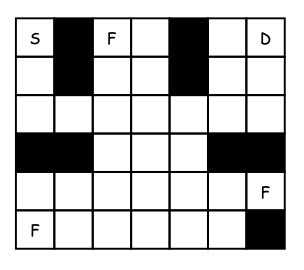
\includegraphics[width=0.25\textwidth]{taxi.png}
\end{figure}

Environment (\cite{dearden1998bayesian}):
In this experience, s is the starting position, d is the destination, and f represents passenger, it will get +1 reward for delivering one passenger, +3 for two , +15 for three.
\\
\\
We preform SARSA with epsilon-greedy, SARSA with Boltzmann softmax and SARSA with Mellowmax softmax. In this environment, there are 33 posible positions and three passengers, therefore, it has 33*2*2*2 = 264 states and four possible actions.
\\
\\
In our algorithm, we set some prohibited state-action pair's Q values to negative infinity, like hit the wall. Moreover, durning the training period, we will not choose those action in order not to affect other Q values.
\\
\\
Because this environment need to have proper exploration, therefore, Boltzmann and Mellowmax can show their advantage. However, there are some detail that not be mention in this paper, so we have our own setting.
\\
\\
In epsilon-greedy method, training and testing both use epsilon-greedy to select action. And in Boltzmann softmax, training and test both use Blotzmann too. However, in Mellowmax softmax, we use Mellowmax softmax durning training process, and in testing process, we select the actions which have max Q values according to our pre-train Q values. We found that there are more approximate to paper's results.

% ==================================================================================
\subsection{Lunar Lander Domain}
\subsection*{Experiment Settings}
The paper's settings:
\begin{itemize}
    \item network: a hidden layer comprised of 16 units with RELU activation functions + a second layer with 16 units and softmax activation functions
    \item use REINFORCE to train the network
    \item batch episode size: 10
    \item learning rate = 0.005
    \item optimizer: Adam
    \item do 10 experiments
    \begin{itemize}
        \item Boltzmann softmax: $\beta=1,2,3,5,10$
        \item Mellowmax: $\omega=3,5,7,8,11$
    \end{itemize}
    \item each experiments do 400 runs, each runs train 40000 episodes
\end{itemize}
Our expiriment settings are basically the same as the paper's, the only different is we do each experiment 3 runs (seed=22, 321, 7654), each run trains 15000 episodes.
Because the training needs a lot of time, so we simplified this part.
